\chapter{Literatur}
	\section{Verwandte Arbeiten}
		\subsection{PointNet}
			Das 2017 in \cite{PointNet} vorgestellte PointNet ist ein neuronales Netzwerk zum Auswerten von Punktwolken. Das Netz bietet dabei sowohl eine Architektur zur Klassifizierung als auch eine zur Segmentierung von Punktwolken. Der Strukturelle Aufbau ist in Abbildung \ref{fig:pointnet} dargestellt. 
			\begin{figure}
				\centering
				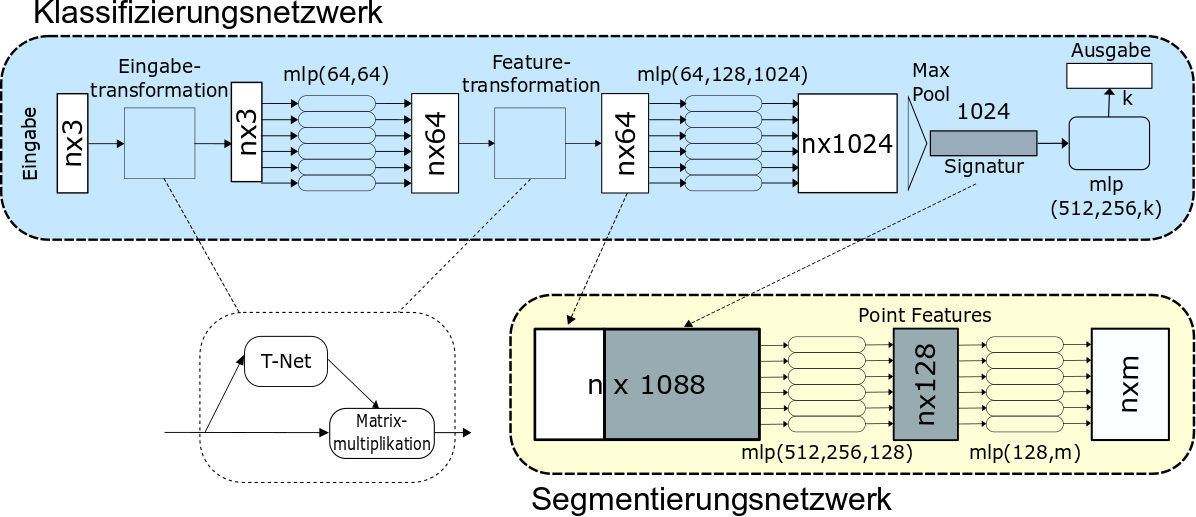
\includegraphics[width=15cm]{img/PointNet.png}
				\caption{Funktionsweise von PointNet}
				\label{fig:pointnet}
			\end{figure} 
			Das Netzwerk erzeugt aus einem Eingabevektor, der aus einer Menge von Koordinaten-Vektoren gebildet wird zun�chst durch Feature Transformation eine globale Signatur, also einen Feature Vektor, der unabh�ngig von der Reihenfolge der Eingabegr��en ist. Um Invarianz bez�glich bestimmter r�umlicher Transformationen wie z.B. Rotation zu erreichen, wird mit einem kleinen neuronalen Netz, dem "`T-Net"', eine Transformationsmatrix angen�hert und auf die Eingabedaten angewandt. Mit der Ausgabe dieses Netzes kann ein weiteres Netz trainiert werden, das diese klassifiziert. Soll das Netzwerk eine Segmentierung der Punktwolke vornehmen, wird der globale Feature Vektor mit dem Eingabevektor kombiniert, um einen Vektor zu erzeugen, der sowohl globale als auch lokale Features repr�sentiert. Anschlie�end kann ein Label f�r jeden Punkt gesch�tzt werden.
			
		\subsection{UPSNet}
			Das 2019 in \cite{UPSNet} vorgestellte UPSNet (Unified Panoptic Segmentation Network) ist ein neuronales Netz f�r panoptische Segmentierung. Dazu f�hrt das Netzwerk parallel eine semantische Segmentierung und eine Instanzsegmentierung des Eingabebildes durch und erstellte mit den kombinierten Ausgaben beider Methoden einen Tensor von Wahrscheinlichkeiten f�r jede Klasse und Instanz. Aus diesem Tensor wird in einem letzten Schritt ein Ausgabebild erzeugt. Der Aufbau des Netzwerks ist in Abbildung \ref{fig:upsarc} dargestellt.\\
			\begin{figure}
				\centering
				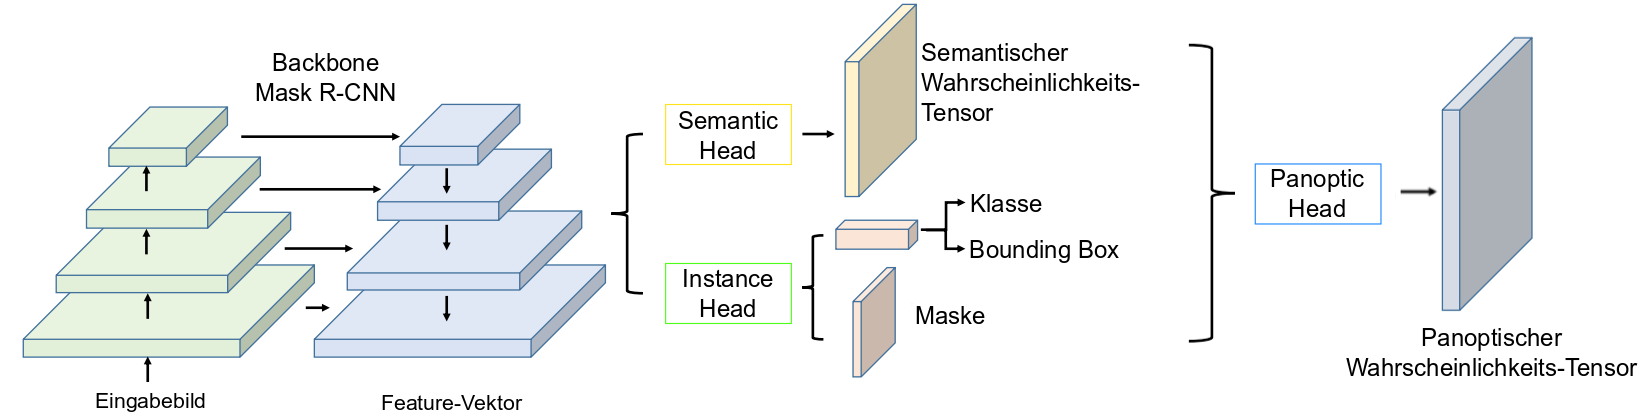
\includegraphics[width=15cm]{img/UPSNet.png}
				\caption{Architektur von UPSNet}
				\label{fig:upsarc}
			\end{figure} 
			UPSNet verwendet als Backbone das in \cite{MaskRCNN} beschriebene Mask R-CNN, das sich aus einem ResNet ableitet. Die Ausgabe des Backbones wird von zwei leichtgewichtigen Netzen, dem "`Semantic Segmentation Head"', der semantisch segmentiert und dem "`Instance Segmentation Head"', der eine Instanzsegmentierung durchf�hrt unabh�ngig voneinander weiterverarbeitet. Die so entstandenen Ergebnisse werden von dem "`Panoptic Segmentation Head"' anhand einer Heuristik ausgewertet, um die Netzwerkausgabe zu erstellen.